\documentclass[12pt]{article}
\usepackage{amsmath,amsfonts,times}
\usepackage{graphicx,color,tikz,pgfplots}
\usepackage[paperwidth=10.1cm,paperheight=6.1cm,lmargin=0in,rmargin=0in,tmargin=0.in,bmargin=0.in]{geometry}
\usepackage{bm}
\usetikzlibrary{arrows,shadings,shapes.arrows,decorations.pathreplacing,calc, positioning}
\usepgfplotslibrary{fillbetween}

\begin{document}
\centering
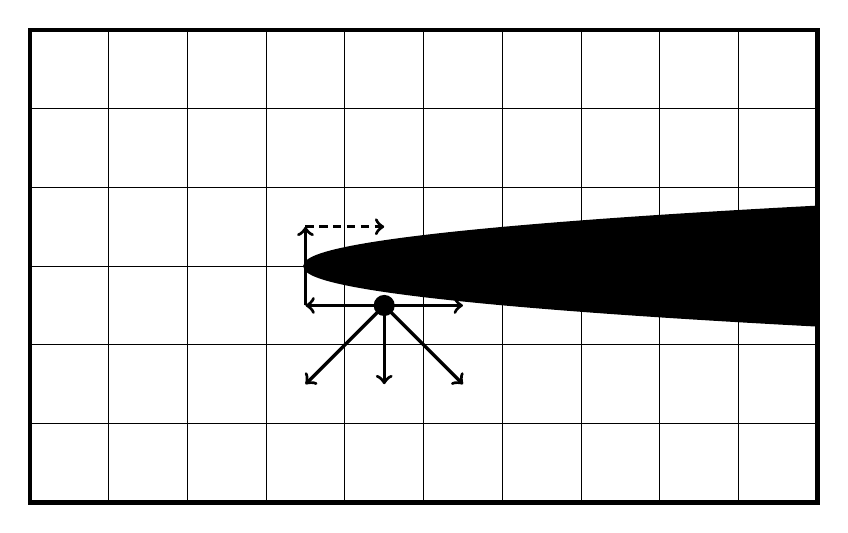
\begin{tikzpicture}[on grid]

  % Parent grid
  \draw[step=10mm, black, thin] (0,0) grid  (10,6); %defining grids
  \draw[black,ultra thick] (0,0) rectangle (10,6);%marking borders


  \clip(0,0) rectangle (10,6);
  \draw[black, ultra thick, draw=black, fill=black, fill opacity=1.0] (53.5,3.0) ellipse (50cm and 1.5cm);
  \draw[black, ultra thick, draw=black, fill=black] (4.5, 2.5) circle (3pt);

  \draw[very thick, black, ->] (4.5,2.5) --++(1,-1);
  \draw[very thick, black, ->] (4.5,2.5) --++(1,0);
  \draw[very thick, black, ->] (4.5,2.5) --++(0,-1);
  \draw[very thick, black, ->] (4.5,2.5) --++(-1,-1);
  \draw[very thick, black, ->] (4.5,2.5) --++(-1,0);
  \draw[very thick, black, ->] (3.5,2.5) --++(0,1);
  \draw[very thick, densely dashed, black, ->] (3.5,3.5) --++(1,0);

\end{tikzpicture}

\end{document} 
